\subsection{Region transition probability}


Based on the definition of dense region and sparse region are recognized. By dividing the region within the Fifth Ring Road, Beijing, China, about $750 km^2$, into $100*100$grids and utilizing the GPS records from March 3,2011 to March 7,2011, regions are recognized. Every cell is regarded as square with length about $274m$. Since area size will affect the area transition probability,a single dense area cannot be larger than 100 cells.
The node dense threshold is set as 121, which is the average node number in the top 5000 dense cells.  Shown as  fig.\ref{figure_dense_area},156 dense areas are recognized and marked by different colors, and the white area is regarded as the sparse area.
%%ÿ���ֲ���ͷһ��Ҫ��&���ţ�����\qquad Ϊ��ո�����

\begin{equation}\label{cell}
\begin{array}{c}
CELL_{x,y}::=\{(lon,lat)|x \le \frac{{lon}}{{len_x}} < x + 1,\\
y \le \frac{{lat}}{{len_y}} < y + 1\}
\end{array}
\end{equation}

\begin{equation}\label{region}
  \begin{array}{r}
REGION_m:: = \{ CEL{L_{x,y}}|\exists CELL_{i,j} \in REGION_m\\
\Rightarrow \|x - i\| \le 1,\|y - j\| \le 1\}
\end{array}
\end{equation}


$p_{i\rightarrow j}^{0\rightarrow 1}$
$p_{i\rightarrow j}^{1\rightarrow 0}$
\begin{figure}[htbp]
\centering
\subfigure[passenger off event regions]{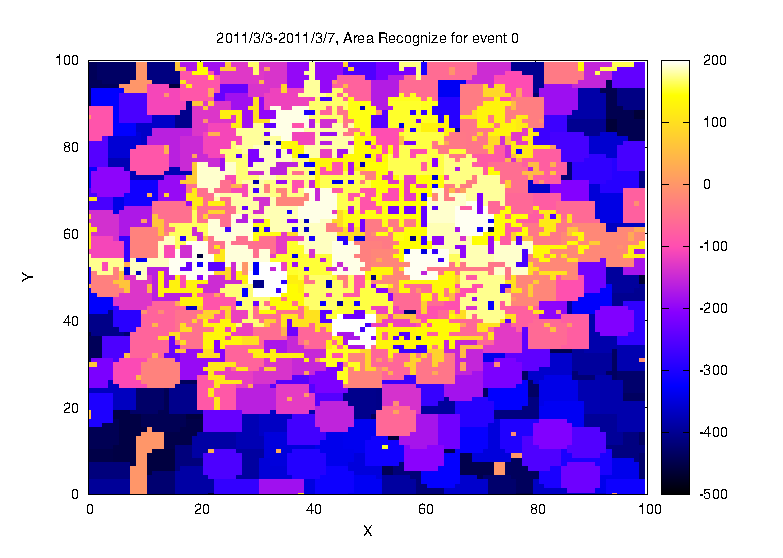
\includegraphics[width=0.4\textwidth]{figures_201103/region/Areas-2011_event0.eps}}
\subfigure[passenger on event regions]{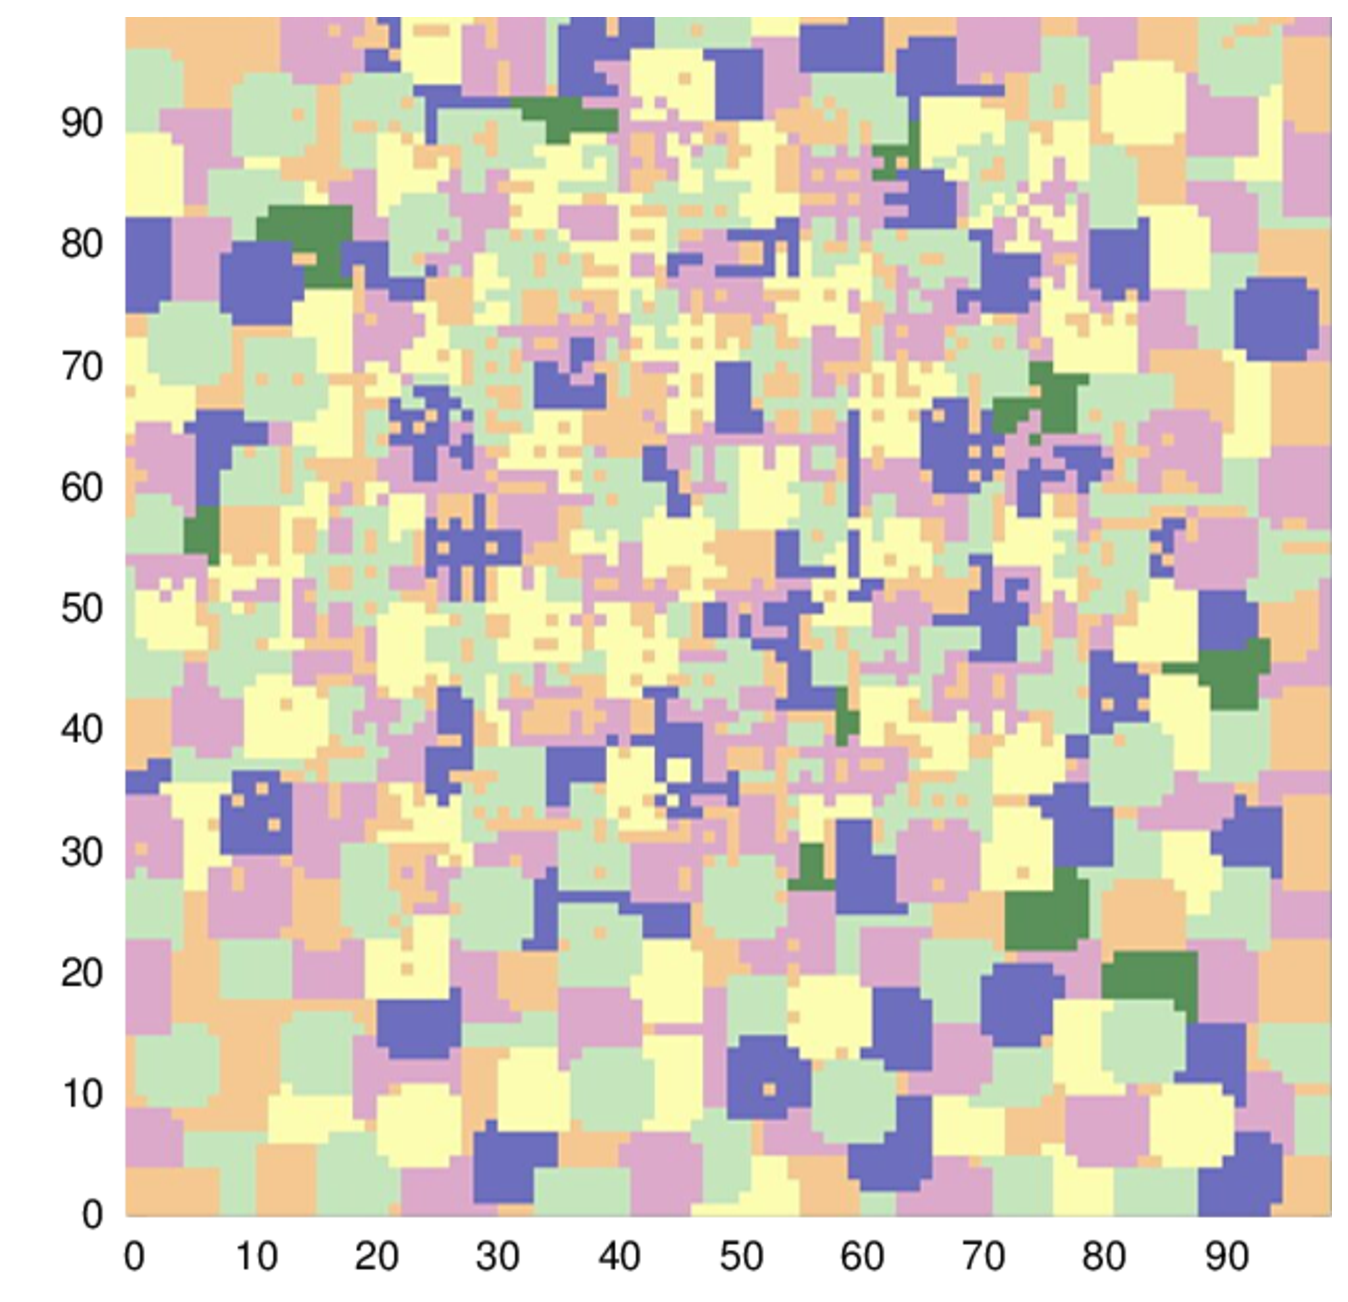
\includegraphics[width=0.4\textwidth]{figures_201103/region/Areas-2011_event1.eps}}
\centering
\caption{Region recognition}\label{figure_region_recognizition}
\end{figure}


A car's trajectory can be regarded as a markov process, and the markov chain nodes are the areas in the city.
This section introduces how to adopt step transition probability matrix from the real trajectory data set.

        After region recognition, n regions including dense regions and a sparse region, can be adopted and marked as $A_i$.  For every short time $\triangle t$, a snapshot of the trajectory is token, which indicates the position information and their area id at time $t$, So that the taxi set for $A_i$ at time $t$ can be found, donated as $TaxiSet^{(t)}_i$. All the taxi set for $k$ time slots and $n$ areas can be presented as a matrix as matrix (\ref{equation_taxiset_matrix}) .
\begin{equation}\label{equation_taxiset_matrix}
\left(
\begin{array}{cccc}
TaxiSet^{(1)}_1 &  TaxiSet^{(2)}_1 & \cdots & TaxiSet^{(n)}_1\\
TaxiSet^{(1)}_2 &  TaxiSet^{(2)}_2 & \cdots & TaxiSet^{(n)}_2 \\
\cdots & \cdots & \cdots & \cdots \\
TaxiSet^{(1)}_k &  TaxiSet^{(2)}_k &  \cdots  & TaxiSet^{(n)}_k \\
\end{array}
\right)
\end{equation}

The One-step transition probability from area $i$ to area$j$, donated as $p_{ij}$, can be calculated by the matrix (\ref{equation_taxiset_matrix}). $|TaxiSet^{(t)}_i|$ means the taxi number in area $i$ at time $t$ and $TaxiSet^{(t)}_i\bigcap TaxiSet^{(t+1)}_j$ is the node number moving from area $i$ to area $j$ in one step$(1\leq m \leq k-1, m\in N^{+} )$.  In that case, $p_{ij}$  during k time slots can be calculated by the formula (\ref{equation_p_ij}):


\begin{equation}\label{equation_p_ij}
\begin{array}{rcl}
  p_{ij}& =&{ {|TaxiSet^{(1)}_i\bigcap TaxiSet^{(2)}_j|+\cdots + |TaxiSet^{(k-1)}_i\bigcap TaxiSet^{(k)}_j|}\over {|TaxiSet^{(1)}_i|+|TaxiSet^{(2)}_i|+\cdots+|TaxiSet^{(k-1)}_i|}} \\
  &=& {\sum_{m=1}^{k-1} |TaxiSet^{(m)}_i\bigcap TaxiSet^{(m)}_j|\over \sum_{m=1}^{k-1}|TaxiSet^{(m)}_i|}\\
  \end{array}
\end{equation}

Note that , $\sum_{j=1}^np_{ij}=1 $ and $p_{ij}\neq p_{ji}$. Then, One-step transition probability matrix is donated as (\ref{equation_taxiset_matrix}) :

\begin{equation}\label{equation_taxiset_matrix}
\textbf{\emph{P}}=(p_{ij})_{n*n}=
\left(
\begin{array}{cccc}
p_{11}&p_{12}&\cdots & p{1n} \\
p_{21}&p_{22}&\cdots & p{nn} \\
\cdots & \cdots & \cdots & \cdots \\
p_{n1}&p_{n2}&\cdots & p{nn} \\
\end{array}
\right)
\end{equation}

